\documentclass[25pt, a0paper, portrait, margin=10mm, innermargin=15mm,
blockverticalspace=15mm, colspace=15mm, subcolspace=8mm]{tikzposter}
\usepackage{natbib}
%\usepackage{pgfplots}
\usepackage[default]{lato}
\usepackage{concrete}
\usepackage[utf8]{inputenc}
\usepackage{graphics}
%\pgfplotsset{/pgf/number format/use comma,compat=1.7}

\definecolor{blau1}{RGB}{0,105,170}
\definecolor{blau2}{RGB}{80,170,200}
\definecolor{rot}{RGB}{198,24,38}
\definecolor{sand}{RGB}{244,241,234}
\definecolor{braun}{RGB}{89,13,8}
\definecolor{green}{RGB}{77,175,74}
\definecolor{red}{RGB}{228,26,28}
\definecolor{purple}{RGB}{152,78,163}
\definecolor{blue}{RGB}{55,126,184}
\tikzstyle{nonterm}=[rounded corners,draw=blue!50,fill=blue!20,thick,font=\sffamily]
\tikzstyle{vroot}=[rounded corners,draw=gray!50,fill=gray!20,thick,font=\sffamily]
\tikzstyle{nontermedge}=[line width=1.5pt,draw=black!50]
\tikzstyle{vrootedge}=[line width=1.5pt,draw=gray!20]
\tikzstyle{termcell}=[matrix,inner sep=1pt,row sep=0pt,matrix anchor=north west]
\tikzstyle{terminal}=[rectangle,font=\small]
\tikzstyle{edgelabel}=[rectangle,draw=gray!50,fill=gray!20,font=\sffamily\tiny]

\usecolorstyle[colorTwo=braun,colorThree=sand,colorOne=rot]{Australia}

\titlegraphic{
\includegraphics[height=10cm]{logo-University-of-Heidelberg.jpg}}
\title{Rule-based Corefence Resolution with BART}
\institute{Institute for Computational Linguistics, Univ. Heidelberg}
\author{Julian Baumann, Xenia Kühling, Sebastian Ruder}
\makeatletter
\makeatother

\begin{document}\maketitle
\begin{columns} \column{0.5}
\block{Goal}
	{	
Integrate rule-based, entity-centric Stanford sieve architecture in BART machine learning system
	} %\note[targetoffsetx=.15\textwidth,targetoffsety=4.5cm,innersep=.4cm,angle=245]{Optional...}
\block{BART}
	{
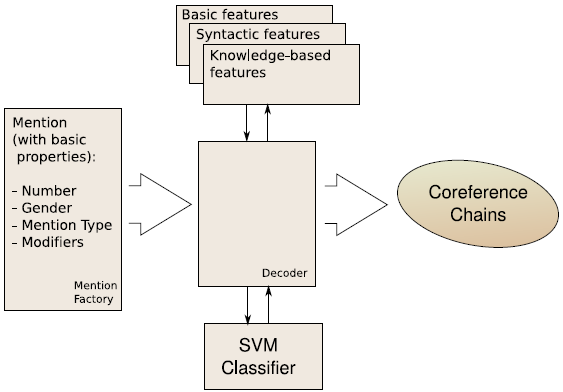
\includegraphics{bart_summary.png}
	}
\block{Blocks}{Blocks are...} %\note[targetoffsetx=-1cm, targetoffsety=-10cm,rotate=5,angle=270,radius=8cm,width=.35\textwidth,innersep=.4cm]{Youcan...}


\block{Evaluation}
	{
\begin{tabular}{l||ll|l}
& \multicolumn{3}{c}{\textbf{MUC-Score}} \\ \hline
               & \textbf{Recall}		 & \textbf{Precision} & \textbf{F\_1}    \\ \hline
Unser System 	& 0.644      & 0.691              & 0.667  \\
BART  & 0.721 		 & 0.532     & 0.612
\end{tabular}
Vergleich mit BARTs Machine Learning-Konfiguration (\texttt{XMLExperiment})

\begin{tabular}{l||ll|l}
& \multicolumn{3}{c}{\textbf{MUC-Score}} \\ \hline
	                 & \textbf{Recall} & \textbf{Precision} & \textbf{F\_1} \\ \hline
SpeakerIdentification & 0.004 & 0.637 & 0.008 \\
+StringMatch & 0.157 & 0.857 & 0.265 \\
+RelaxedStringMatch & 0.180 & 0.825 & 0.295 \\
+PreciseConstructs & 0.241 & 0.822 & 0.372 \\
+HeadMatchA & 0.295 & 0.809 & 0.432 \\
+HeadMatchB & 0.355 & 0.775 & 0.487 \\
+HeadMatchC & 0.357 & 0.771 & 0.488 \\
+ProperHeadNounMatch & 0.358 & 0.771 & 0.489 \\
+RelaxedHeadMatch & 0.383 & 0.771 & 0.512 \\
+PronounMatch & 0.644 & 0.691 & 0.667 \\ 
\end{tabular}
Performanz der einzelnen \textit{sieves}

\begin{tabular}{l||ll|l}
& \multicolumn{1}{c}{\textbf{MUC-Score}} \\ \hline
          &    \textbf{F\_1}    \\ \hline
Unser System &	  0.420  \\
Stanford   &	0.603
\end{tabular}
Vergleich mit dem Stanford-System
	}

\column{0.5} \block{Columns}{By default,...}
\begin{subcolumns} \subcolumn{.4} \block{Subcolumns}{If you...} \subcolumn{.5} \block{}{An example...} \end{subcolumns}
\block[titlewidthscale=.8,bodywidthscale=.9,titleoffsety=7.5mm,bodyoffsety=7mm]{Changing the Poster’s Appearance}{If the default...}
\block{Stanford}
{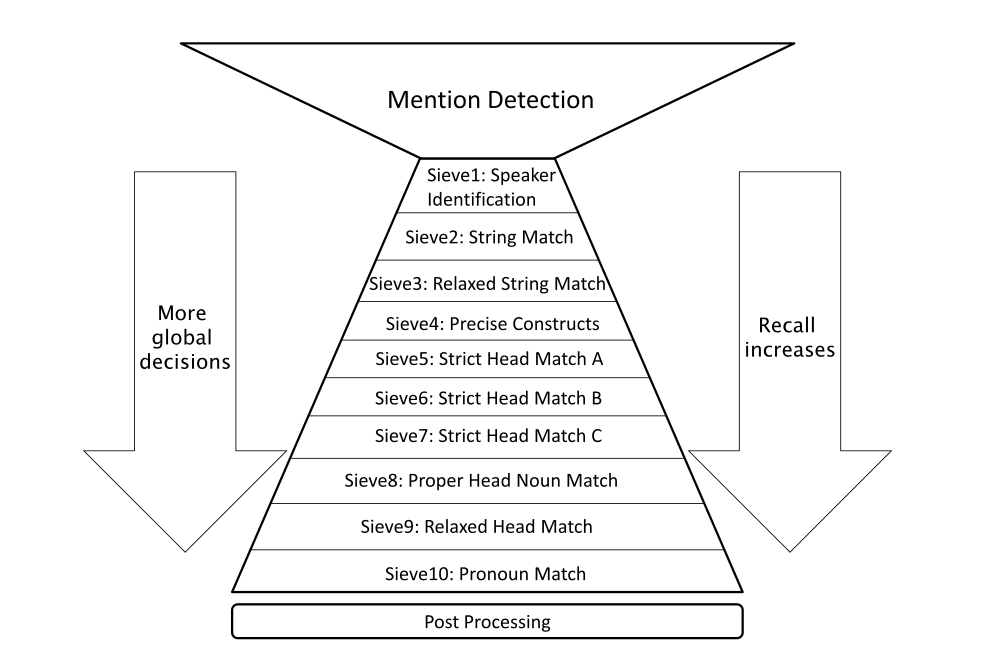
\includegraphics{stanford.png}}

\block{Conclusion}
	{
The rule-based sieve approach exceeds ML performance. Because our system has been designed primarily using linguistic constants specific to German, there still remains a lot of room for improvement for the English language. Due to the nature of the rule-based approach, the system is easy to extend. We leave this along with its adaptation to English, Italian, and other languages as future work.
	}
\end{columns}

\end{document}
